\section{Lógica}

\begin{questions}

\question Considere las siguientes premisas: 
\begin{enumerate}[I.]
    \item Toda conferencia es discurso. 
    \item Algunas conferencias no son lecciones. 
\end{enumerate}
De las premisas anteriores se sigue que: \footnote{\cite{TEC2023}}
\begin{choices}
    \choice Ninguna lección es discurso. 
    \choice Todas las lecciones son discursos. 
    \CorrectChoice Algunos discursos no son lecciones. 
    \choice Todos los discursos son conferencias.
\end{choices}

\begin{solution}
    Podemos verlo en un diagrama de Venn. Como toda conferencia es discurso, el area que representa las conferencias está adentro del area que representa los discursos. A su vez, como algunas conferencias no son lecciones, eso quiere decir que hay una parte de las conferencias que no está dentro de las lecciones:
    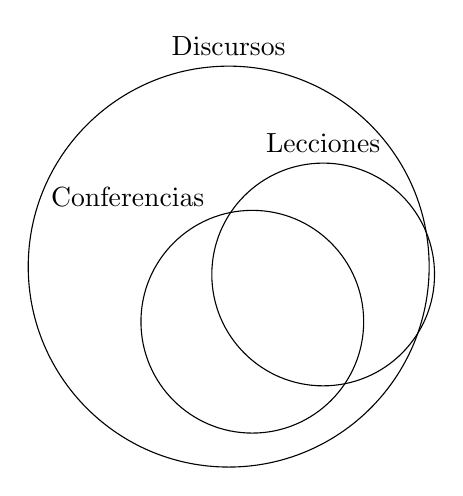
\begin{tikzpicture}
        \node [circle, draw, inner sep =1cm, label=110:Conferencias] at (0.3,0) {};
        \node [circle, draw, inner sep =1.8cm, label=90:Discursos] at (0,0.7) {};
        \node [circle, draw, inner sep =1cm, label={90:Lecciones}] at (1.2,0.6) {};
    \end{tikzpicture}
    El diagrama no muestra todas las posibles situaciones. Sin embargo, lo más importante es que conferencias está dentro de discursos, y que lecciones no cubre todo conferencias, porque hay conferencias que no son lecciones. Con esta intuición, vemos que podrían haber lecciones que sean discursos, luego la A. no es. Además, podrían haber lecciones que no sean discursos. Eso tampoco lo sabemos, la B. no es.

    ¿Será que siempre hay algunos discursos que no son lecciones? En el dibujo así lo parece, pero pensemos, si todo discurso fuera lección, entonces como toda conferencia es discurso, necesariamente toda conferencia sería lección, por lo que esto no puede pasar. Por lo tanto, algunos discursos --- en particular los que son conferencias que no son lecciones --- no son lecciones. La C. es la respuesta correcta.

    Para completar, vemos que aunque toda conferencia sea discurso, podrían haber discursos que no sean conferencias, entonces la D. no es. \hfill $\square$
\end{solution}

\question Considere las siguientes premisas:
\begin{enumerate}[i)]
\item Todos los ciervos tienen cuernos.
\item Algunos rumiantes son ciervos.
\end{enumerate}
De las premisas anteriores se sigue que \footnote{\cite{TEC2023}}
\begin{choices}
    \choice algunos ciervos no son rumiantes.
    \CorrectChoice algunos rumiantes tienen cuernos.
    \choice todos los rumiantes tienen cuernos.
    \choice algunos rumiantes no tienen cuernos.
\end{choices}

\begin{solution}
    Por la segunda premisa, hay rumiantes que son ciervos. Tomemos uno y digamos que se llama Steve. Como Steve es un ciervo, por la primera premisa tiene cuernos. De esta forma Steve es un rumiante ciervo con cuernos. Esto nos pemite concluir con certeza que algunos rumiantes tienen cuernos. La B. es la opción correcta.

    Pensemos por qué las demás no son correctas. Es importante considerar que cuando una opción no es correcta, no significa que sea falsa siempre, sino que existen escenarios donde es falsa. La A. podría ser pero podría no ser. Es perfectamente posible que todos los ciervos sean rumiantes, y eso no contradice las premisas.

    Para la C., solo sabemos que algunos rumiantes son ciervos, así que podría existir un rumiante Patricio que no sea ciervo, y como no es ciervo, podría no tener cuernos, no sabemos con certeza.

    La D. tampoco podemos afirmarla con certeza. Podría suceder que todos los rumiantes fueran ciervos, en cuyo caso todos tienen cuernos. O podría pasar que, aunque algunos rumiantes no fueran ciervos, de igual forma tengan cuernos. No nos dicen que solo los ciervos tengan cuernos \hfill $\square$
\end{solution}

\question Considere las siguientes premisas:
\begin{enumerate}[i)]
\item Si V lee, entonces L dibuja o J salta.
\item Si L dibuja, entonces P no corre.
\item L no dibuja y J no salta.
\end{enumerate}
De las premisas anteriores se sigue que \footnote{\cite{TEC2023}}
\begin{choices}
    \choice V lee.
    \choice P corre.
    \CorrectChoice V no lee.
    \choice P no corre.
\end{choices}

\begin{solution}
    Analicemos las opciones:
    \begin{enumerate}[A.]
        \item Si V lee, por la premisa i) tendríamos que L dibuja o J salta. Pero la premisa iii) nos dice que L no dibuja y J no salta. Por lo tanto, no puede ser cierto que V lee. De hecho, justamente por esto podemos afirmar que V no lee, es decir que la respuesta C. es la correcta.
        \item ¿Podemos estar seguros de que P corre? Por la premisa ii), si P corre, entonces L no dibuja (si dibujara sabríamos que P no corre), y esto coincide con la iii). Sin embargo, también podría ocurrir que aunque L no dibuja, que P no corre, pues sabemos que si L dibuja entonces P no corre, pero esto \textbf{no implica} que si L no dibuja entonces P sí corre. 
        
        Para poner un ejemplo, un papá le puede decir a su hijo: si ganas la carrera te doy un premio. Y el hijo se esfuerza pero al final no gana. Sin embargo, el papá igual le da un premio por su esfuerzo. Ahí, el papá dijo: Si ganas, te doy un premio. Pero esto no implica que: Si no ganas, no te doy un premio. En el caso en el que no gana, el papá puede hacer lo que quiera.
        
        Así mismo en este caso, si L no dibuja, la premisa ii) no nos dice nada sobre si P corre o no corre, pues solo nos da información cuando L dibuja.

        Así, no podemos afirmar con certeza que P corre o que P no corre. Así, la B. y la C. no son correctas, no se siguen de las premisas.
        \item Esta es la correcta. Ver el comentario a A.
        \item Ver comentario a B.
    \end{enumerate}
    \hfill $\square$

    {\small \itshape
    Esta puede ser una buena ocación para introducir el concepto de contrapositiva. Si tenemos una premisa de la forma ``Si P entonces Q,'' y sabemos que Q no es cierto, entonces podemos concluir que P no es cierto. Es decir, las afirmaciones ``Si P entonces Q'' y ``Si Q no es cierto entonces Q no es cierto'' son equivalentes.

    En este ejercicio, ¿cuál es la contrapositiva de i)? ``Si no es cierto que L dibuje ni que J salte, entonces V no lee''. O, escribiendola mejor ``Si L no dibuja y J no salta entonces V no lee''. Y entonces queda muy claro que por la iii) como L no dibuja y J no salta, entonces necesariamente V no lee.}
\end{solution}

\question Considere las siguientes afirmaciones:
\begin{enumerate}
    \item Si Luciana se pegó la lotería, Alejandro no está en el parque.
    \item Si Alejandro está en el parque, Carlos no fue a clases hoy.
    \item Carlos fue a clases hoy.
\end{enumerate}
Si las afirmaciones anteriores son verdaderas, se concluye con certeza que

\begin{choices}
    \choice Luciana se pegó la lotería.
    \choice Alejandro está en el parque.
    \CorrectChoice Alejandro no está en el parque. %%%
    \choice Carlos está en la universidad.
    \choice Luciana es la madre de Alejandro.
\end{choices}

\begin{solution}
    Reescribamos las proposiciones como L: ``Luciana se pegó la lotería'', A: ``Alejandro está en el parque'' y C: ``Carlos fue a clases''. Entonces las premisas son 
    \begin{enumerate}[i)]
        \item Si L entonces no es cierto que A.
        \item Si A entonces no es cierto que C.
        \item C sí es cierto.
    \end{enumerate}
    Entonces vemos claro que como C sí es cierto (Carlos si fue a clases), entonces A no es cierto por la contrapositiva de ii) (de nuevo, si Alejandro estuviera en el parque, entonces Carlos no fue a clases, pero Carlos sí fue a clases). La i) no nos dice mucho, pues si L es cierto (que Luciana se pegó la lotería) entonces no es cierto que A, que ya lo sabemos, y si L no fuera cierto, de nuevo, podría pasar cualquier cosa, que A esté en el parque o no. 

    Por esto, lo que sabemos con certeza es que Carlos fue a clases y que Alejandro no está en el parque. Así, la opción C. es la correcta. \hfill $\square$
\end{solution}

\question Gabriel, Elena, Ignacio y Susana se reunieron para realizar una carrera de velocidad. Al final de la carrera sucedió que: 
\begin{enumerate}[i)]
\item Gabriel llegó a la meta antes que Susana. 
\item Elena llegó a la meta antes que Ignacio. 
\item Gabriel llegó a la meta antes que Ignacio. 
\end{enumerate}

¿En qué posiciones pudo haber llegado Gabriel?  \footnote{\cite{practicaUCR1}} 
\begin{choices} 
\CorrectChoice En la primera o la segunda. 
\choice En la primera o la tercera. 
\choice En la segunda o la tercera. 
\choice En la segunda o la cuarta.
\end{choices}

\begin{solution}
    Tenemos que ordenar a los participantes. Digamos que A $<$ B si A llegó antes que B. Si a cada participante lo denotamos por su inicial, sabemos que G $<$ S, que E $<$ I y que G $<$ I y nos preguntan en qué posición pudo haber quedado Gabriel. Por el contexto, podemos asumir que solo ellos 4 participaron en la carrera. Y como Gabriel le ganó a dos de ellos, tuvo que haber quedado en la primera o en la segunda posición.

    La opción correcta es la A. \hfill $\square$
\end{solution}

\question Se tienen tres lapiceros X, Y y Z: dos son verdes y uno es rojo; además, X y Y son de diferente color. Considere las siguientes proposiciones:
\begin{enumerate}[I.]
\item Y es verde
\item Z es verde
\item X es verde
\end{enumerate}

De las anteriores, ¿cuáles se cumplen con certeza? \footnote{\cite{practicaUCR1}} 

\begin{choices}
    \CorrectChoice Solo II %%%%%%%%
    \choice Solo III
    \choice II y III
    \choice I y II  
\end{choices}

\begin{solution}
    Como $X$ y $Y$ son de distinto color, alguno de los dos es verde y el otro es rojo, pero no estamos seguros de cuál es cual. Lo que sí sabemos es que solo hay un lapicero rojo. Como este debe ser X o Y, no puede ser Z. De esta forma, con certeza Z no es rojo y por lo tanto debe ser verde. La opción correcta es la A. Solo II., pues no podemos tener \textbf{certeza} de que Y sea verde o de que X sea verde, aunque alguna de las dos sí tiene que pasar: no sabemos cuál de las dos. \hfill $\square$
\end{solution}

\question Fabio tiene 12 balones de futbol, 8 balones de volibol y 3 balones de basketbol en una canasta. Desde una habitacion distinta, Fabio pone a un robot a sacar una cantidad de balones de manera aleatoria. ¿Cuál es el mínimo de balones que debe pedir Fabio al robot para tener certeza de que, sin importar cuales balones saque, al entrar a la habitación vea al menos un balón de cada deporte fuera de la canasta?


\begin{choices}
\CorrectChoice 21 balones %%%
\choice 12 balones
\choice 16 balones
\choice 23 balones
\choice 3 balones
\end{choices}

\begin{solution}
    Esta es una pregunta de encontrar el peor caso posible. Es decir, preguntarse, ¿en qué situación el robot pudo haber sacado un montón de balones, pero que aún no haya sacado un balón de alguno de los deportes?

    Porque claramente si tiene suerte puede sacar, de una vez, uno de cada tipo de balón distinto y ya tener los tres, pero esto no ocurre con certeza.

    Si saca todos los balones, con certeza habrá uno de cada tipo de balón, pero... ¿se podrá tener esta certeza con menos?

    Si saca todos los balones excepto uno, como hay 12 balones de futbol, 8 de voli y 3 de basket, sin importar si quedó uno adentro de alguno de los deportes, habrá uno afuera, pues hay más de uno de cada tipo. Fabio puede seguir teniendo certeza de que hay uno de cada deporte fuera de la canasta.

    Lo mismo podemos decir si quedan 2 dentro de la canasta, pues hay al menos 3 de cada deporte. 

    Sin embargo, si quedaran 3 dentro de la canasta es posible que sean los tres balones de baloncesto los que queden dentro de la canasta, y no hay ninguno fuera. Por lo tanto, si Fabio pide al robot que saque 20 balones, podría sacar todos los de futbol que son 12 y todos los de voli que son 8, pero no sacar ni uno de baloncesto. 
    
    Por lo tanto, para tener certeza de que hay al menos un balón de cada tipo de deporte fuera de la canasta Fabio debe pedir al robot que saque al menos 21 balones. La opción correcta es la A. \hfill $\square$
\end{solution}

\question Un grupo de personas quiere comenzar a practicar algún deporte que sea adecuado a sus preferencias y habilidades, de manera que nadie se quede sin practicar uno o más deportes. A partir de estos requisitos, se toman en cuenta los siguientes aspectos:

\begin{enumerate}[I.]
    \item A todos les gusta mojarse y no saben andar en bicicleta.
    \item Todos pueden mantenerse a flote en el agua y no les gusta el contacto físico.
    \item Algunos pueden controlar bien los objetos esféricos y no desean recorrer largas distancias.
\end{enumerate}

De acuerdo con los aspectos anteriores, ¿qué se puede concluir, con certeza? \footnote{\cite{60-10preguntas}} 
    \begin{choices}
        \choice Algunos pueden practicar natación y ciclismo.
        \choice Todos pueden practicar ciclismo, pero no boxeo.
        \CorrectChoice Todos pueden practicar natación, pero no ciclismo.
        \choice Algunos pueden practicar boxeo y todos pueden practicar natación. 
    \end{choices}

\begin{solution}
    Veamos las opciones.
    \begin{enumerate}[A.]
        \item ¿Algunos pueden practicar natación y ciclismo? La premisa I. nos dice que no saben andar en bicicleta, y esto aplica para todos. Por lo tanto ninguno puede practicar ciclismo.
        \item ¿Todos pueden practicar ciclismo? De nuevo: no saben andar en bici.
        \item ¿Todos pueden practicar natación, pero no ciclismo? La premisa I. nos dice que a todos les gusta mojarse y la II. que todos pueden mantenerse a flote en el agua. Por tanto, todos pueden practicar natación. Al mismo tiempo, la I. nos dice que no saben andar en bicicleta, por lo que no pueden practicar ciclismo. Por lo tanto, esta es correcta.
        \item ¿Algunos pueden practicar boxeo y todos pueden practicar natación? Es cierto que todos puede praticar natación. Pero la II. nos dice que no les gusta el contacto físico, por lo que no les gustaría el boxeo. Así, esta no puede ser.
    \end{enumerate} 
    La opción correcta es la C. \hfill $\square$
\end{solution}

\question Luis es hijo de la madre de Marta. Marta es la abuela materna de la hija de Ana. Si Luis tiene un hijo llamado Pedro. ¿Qué relación tiene Pedro con el hermano de Ana?

\begin{choices}
    \CorrectChoice Son primos.
    \choice Pedro es su tío.
    \choice Pedro es su sobrino.
    \choice No tienen parentesco.
\end{choices}

\begin{solution}
    Empecemos por la pregunta y vayamos paso a paso. ¿Qué relación tiene Pedro con el hermano de Ana? Pedro es el hijo de Luis, y Ana tiene una hija cuya abuela materna es Marta. Como Ana es la mamá de su hija, Marta, siendo abuela materna, es la mamá de Ana. Para conectarlos, vemos que Luis es hijo de la madre de Marta. Por lo tanto, Marta y Luis comparten mamá, es decir, son hermanos. Así, tenemos el siguiente diagrama:
    
    \begin{center}
        \begin{tikzcd}[column sep=0.5em, row sep = 4ex]
            & \text{Marta} \ar[ld] \ar[rd] \ar[rdd, sloped, "\text{abuela}","\text{materna}"'] \ar[rrd] & \\
            \text{Luis} \ar[d] & & \text{Ana} \ar[d] & \text{Hermano de Ana} \\
            \text{Pedro} & & \text{Hija de Ana}
        \end{tikzcd}
    \end{center}

    Note por tanto que el hermano de Ana debe ser también hijo de Marta y por tanto hermano de Luis. Como Pedro es hijo de Luis, el hermano de Ana (que es hermano de Luis) debe ser tío de Pedro. \hfill $\square$
\end{solution}

\question En una habitación de cuatro paredes, dos tienen una pintura, otra un televisor y la otra está vacía.

Respecto a la ubicación de los objetos, ¿cuál de las siguientes opciones, con certeza, es verdadera? \footnote{\cite{60-10preguntas}} 
\begin{choices}
    \choice Las pinturas están en paredes opuestas.
    \choice Las pinturas están en paredes contiguas.
    \choice El televisor está en una pared opuesta a la pared vacía.
    \CorrectChoice Una pintura está en una pared contigua a la pared vacía. 
\end{choices}

\begin{solution}
    Aqui, lo mejor es ver las opciones e intentar encontrar contraejemplos, casos en los que no son ciertas:
    \begin{enumerate}[A.]
        \item Veamos que podemos poner las pinturas en paredes contiguas sin problema, y un televisor en alguna de las otras paredes, por lo que no es necesario que las pinturas estén en paredes opuestas.
        \item Igual que en la anterior, también es posible que las pinturas estén en paredes opuestas, por lo que no es necesario --- no se sabe con certeza --- que las pinturas estén en paredes contiguas.
        \item El televisor está en una pared opuesta a la pared vacía. Tampoco es necesario. Podemos poner el televisor opuesto a una pintura y por tanto estará contiguo a la pared vacía, que debe ser una de las dos que quedan.
        \item Por último, intentemos hacer que ninguna pintura esté en una pared contigua a la pared vacía, y veamos que no es posible: si una pintura no está contigua a la pared vacía, solo es posible que esté opuesta a esta pared (solo hay cuatro paredes, una será la vacía, otras dos serán contiguas a esta vacía y una será opuesta). ¡Pero tenemos dos pinturas, y solo una pared opuesta a la pared vacía! No podemos poner ambas pinturas en la misma pared. Por lo tanto, aunque pongamos una pintura opuesta a la pared vacía, la otra tendrá que estar contigua a la pared vacía. De esta forma, sabemos con certeza que una pintura está en una pared contigua a la pared vacía. 
    \end{enumerate} 
    La opción correcta es la D. \hfill $\square$
\end{solution}


\question Después de hacer una encuesta en la población A, conformada por 425 mujeres y 325
hombres, se obtiene la siguiente información:
\begin{center}
\centering
\begin{tabular}{|c|c|}
    \hline
    \textbf{Tipo de población} & \textbf{Total}\\
    \hline\hline
    Niños en escuela           & 225 \\
    Jóvenes en el colegio      & 175 \\
    Adultos menores de 65 años & 250 \\
    Adultos mayores de 65 años & 100 \\
    \hline
\end{tabular}
\end{center}
Considere las siguientes afirmaciones:
\begin{enumerate}[I.]
    \item De cada 75 adultos mayores, 13 son mujeres.
    \item Por cada 7 colegiales hay 9 escolares.
    \item De cada 30 escolares, 13 son hombres.
\end{enumerate}
De las afirmaciones anteriores, ¿cuáles se cumplen con certeza? \footnote{\cite{TEC2023}}
\begin{choices}
    \CorrectChoice Solo II %%%%%%%%
    \choice Solo III
    \choice I y II
    \choice II y III
\end{choices}

\begin{solution}
    Veamos las afirmaciones una por una
    \begin{enumerate}[I.]
        \item De cada 75 adultos mayores, 13 son mujeres: Sabemos que hay 100 adultos mayores, que hay en total 425 mujeres y 325 hombres. Sin embargo, con sabemos cómo se distribuye el si son hombres o mujeres. En un caso muy hipotético, solo hay niños varones y hay 100 jóvenes varones, por lo que ya con estos son todos los hombres de la población, y los adultos mayores todos serían mujeres, de cada 75, las 75 son mujeres. Así, no sabemos con certeza que esto ocurre con la información que tenemos.
        \item Por cada 7 colegiales hay 9 escolares: Si tenemos 175 colegiales y 225 escolares. Si agrupamos los colegiales de 7 en 7 obtenemos $175/7 = 25$ grupos, y si agrupamos los escolares de 9 en 9 obtenemos $225/9 = 25$ grupos. Notamos entonces que por cada grupo de 7 colegiales hay un grupo de 9 escolares, pues son la misma cantidad de grupos. De esta forma, esta es una afirmación que se cumple con certeza.

        En otras palabras lo que nos dice esta afirmación es que la razón de colegiales a escolares es igual a $7/9$. I.e., que $175/225=7/9$.

        \item De cada 30 escolares, 13 son hombres: De nuevo, no tenemos información sobre disribución de hombres y mujeres en cada uno de los rangos de edad. Es posible que todos los escolares sean niños, como dijimos en el caso anterior, de forma que no sabemos con certeza que de cada 30 escolares 13 sean hombres.
    \end{enumerate}

    Concluimos que la única afirmación que se cumple con certeza es la II. Así, la respuesta correcta es la A. \hfill $\square$
\end{solution}

\question
En una fábrica se empacan 96 bombillos en cajas de 8. Cada caja debe haber estrictamente más bombillos en perfecto estado que defectuosos. ¿Cuál de las siguientes opciones es imposible que ocurra?
\begin{choices}
  \choice Solo se empacaron 32 bombillos defectuosos.
  \choice Se empacaron más de 48 bombillos en perfecto estado.
  \choice Se empacaron 36 bombillos defectuosos.
  \CorrectChoice Solo se empacaron 55 bombillos en perfecto estado. %%
\end{choices}

\begin{solution}

    Primero, leamos la pregunta ¿cuál de las siguientes opciones es imposible que ocurra? Por tanto, hay 3 que sí pueden ocurrir y solo una que es imposible Como en cada caja hay 8 bombillos y debe haber estrictamente más bombillos en perfecto estado que defectuosos en cada caja, debe haber al menos 5 buenos y como máximo 3 malos en cada caja. ¿Cuántas cajas se producen? $96/8= 12$. Hay 12 cajas. Como cada caja tiene al menos 5 bombillos buenos, hay al menos $12 \cdot 5 = 60$ bombillos buenos. Al mismo tiempo, hay a lo sumo (máximo) $12\cdot 3 = 36$ bombillos malos. Como debe haber al menos 60 bombillos en perfecto estado no es posible que solo se hayan empacado 55.´

    No es difícil ver a partir de nuestro análisis que las otras tres afirmaciones son posibles. Así, la respuesta correcta es la D. \hfill $\square$
\end{solution}

% \question En un torneo participan 6 jugadores X, Y, Z, D, E y F y cada uno se enfrenta a los demás.
% Se asignan tres puntos por cada gane y un punto por cada empate. Gana quien obtenga el mayor puntaje. En caso de empate se disputa otra ronda entre los jugadores empatados para obtener un vencedor.

% La tabla final de resultados tiene la siguiente información:
% \begin{center}
% \begin{tabular}{|c|c|c|c|c|}
%     \hline
%       & Ganados & Empatados & Perdidos & Puntos totales \\ \hline
%     X & 2       &           & 2        &                \\ \hline
%     Y &         & 1         &          & 10             \\ \hline
%     Z &         &           & 2        & 5              \\ \hline
%     D & 2       & 1         &          &                \\ \hline
%     E &         &           &          & 3              \\ \hline
%     F &         & 3         & 0        &                \\ \hline
% \end{tabular}
% \end{center}
% Considere las siguientes afirmaciones:
% \begin{enumerate}[I.]
%     \item D perdió contra X.
%     \item Hay dos jugadores que empatan en puntaje.
%     \item Si F hubiera ganado un partido más, habría ganado el torneo.
% \end{enumerate}
% De las anteriores, ¿cuáles se cumplen con certeza? \footnote{\cite{TEC2023}}
% \begin{choices}
%     \choice Solo I
%     \CorrectChoice Solo II %%%%%%%
%     \choice I y III
%     \choice II y III
% \end{choices}

% \begin{solution}
%     Nos preguntan qué afirmaciones se cumplen con certeza. Tenemos mucha información y es fácil perderse entre tantos datos. Intentemos descubrir si hay datos sencillos de agregar. Cada jugador, como se enfrenta a los demás, jugó al menos 5 veces, posiblemente más si empató con el mayor puntaje. De momento veamos los primeros 5 partidos
%     \begin{itemize}
%         \item Como X ganó 2 partidos y perdió 2, empató uno y tuvo $2\cdot 3 + 1\cdot 1 = 7$ puntos.
%         \item Como Y empató solo un partido y tiene 10 puntos, tuvo que haber ganado exactamente 3 para completar el resto de los puntos. Perdió al menos un partido.
%         \item Como Z tiene 5 puntos y perdió dos partidos, no pudo haber empatado 5 veces, luego ganó una y empató otros dos.
%         \item D tiene $2\cdot 3 + 1\cdot 1 = 7$ puntos. Perdió al menos 2 partidos.
%         \item E tiene 3 puntos. Pudo haber ganado una vez y perdido el resto o empatado tres veces. En todo caso, perdió al menos 2 veces y posiblemente 4 veces.
%         \item F empató tres veces y nunca perdió. Luego tuvo que haber ganado las otras 2 veces, obteniendo al menos $2\cdot 3+ 3\cdot 1 = 9$ puntos.
%     \end{itemize}
%     De momento la tabla va así
% \begin{center}
% \centering
% \begin{tabular}{|c|c|c|c|c|}
% \hline
%   & Ganados & Empatados & Perdidos & Puntos totales \\ \hline
% X & 2       & 1+        & 2        & 7+             \\ \hline
% Y & 3       & 1         & 1+       & 10             \\ \hline
% Z & 1       & 2         & 2        & 5              \\ \hline
% D & 2       & 1         & 2+       & 7              \\ \hline
% E & 1 o 0   & 0 o 3     & 4 o 2    & 3              \\ \hline
% F & 2+      & 3         & 0        & 9+              \\ \hline
% \end{tabular}
% \end{center}
% Recordemos que no tenemos toda la información, simplemente nos preguntan qué sabemos que ocurrió con certeza. ¿Es posible que D no perdiera contra X? Sí, pudo haber ganado contra X o incluso empatado contra él y que el resto de puntos se acomodaran. Sería interesante dar un ejemplo explícito, pero hay suficiente libertad con los datos que tenemos como para construirlo. 

% Hay dos jugadores que empatan en puntaje? Es posible que no. Sabemos los puntos exactos de Y, Z, D y E. 
% \hfill $\square$ \end{solution}

% Revisar
% \question % GPT principio del palomar
% En un vivero hay 92 árboles divididos en tres especies: 42 cenízaros, 30 guanacastes y 20 almendros. Estos árboles serán sembrados por 23 estudiantes, y cada estudiante debe plantar 4 árboles. 

% ¿Cuál de las siguientes afirmaciones se cumple con certeza?
% \begin{choices}
%   \choice Al menos un estudiante plantará 3 cenízaros. %%
%   \choice Al menos un estudiante plantará un guanacaste y un cenízaro.
%   \choice Al menos un estudiante plantará 2 almendros.
%   \choice Al menos un estudiante plantará un arbol de cada tipo.
% \end{choices}

\question Una empresa chocolatera empaca su producción en paquetes con 13 chocolates cada uno. La producción del lunes fue de 195 chocolates. Se sabe que en cada paquete hay más chocolates blancos que chocolates amargos, entonces no es posible que se hayan producido \footnote{Modificado de \cite{SEMA2022}}
\begin{choices}
    \choice 105 unidades de chocolate blanco.
    \CorrectChoice Exactamente 90 unidades de chocolate blanco.
    \choice 90 unidades de chocolate amargo.
    \choice más de 90 unidades de chocolate blanco. 
\end{choices}

\begin{solution}
    Notemos que la pregunta es de imposibilidad: ``\textbf{no} es posible que se hayan producido ...''. 

    En cada paquete hay 13 chocolates, y hay más chocolates blancos que amargos. Por lo tanto, debe haber menos de 6 chocolates amargos (si hubiese una cantidad mayor o igual que 7, entonces quedan menos de 6 chocolates no amargos en el paquete y necesariamente habría más amargos que blancos). ¿Cuántos paquetes se hicieron el lunes? $195/13 = 15$. Por lo tanto: en cada paquete hay 6 chocolates amargos o menos y hay 15 paquetes, luego hay $15 \cdot 6 = 90$ unidades de chocolate amargo o menos.

    De momento esto no contradice ninguna de las opciones. Pero si --- del contexto --- asumimos que solo hay chocolates blancos y amargos, entonces el hecho de que haya máximo 90 chocolates amargos nos dice que hay como mínimo $195-90 = 105$ chocolates blancos. Por lo tanto, no es posible que se hayan producido exactamente 90 unidades de chocolates blanco, pues son menos que las 105 requeridas. 

    La opción correcta es la B. \hfill $\square$
\end{solution}

\question En un vivero hay 60 árboles pequeños de
diferentes tipos: 31 guanacastes, 19 cenízaros y
10 almendros. Los árboles serán sembrados en
una finca por 30 estudiantes. Cada estudiante
sembrará dos árboles.
Según la información anterior, ¿cuál de las
siguientes situaciones ocurrirá con certeza? \footnote{\cite{SEMA2021}}
\begin{choices}
    \choice Uno o más estudiantes sembrarán dos
cenízaros.
    \CorrectChoice Uno o más estudiantes sembrarán dos
guanacastes.
    \choice Uno o más estudiantes sembrarán un
guanacaste y un almendro.
    \choice Uno o más estudiantes sembrarán un
guanacaste y un cenízaro.
\end{choices}

\begin{solution}
    En esta, como en el ejercicio de la habitación con las dos pinturas, la tele y la pared vacía, lo ideal es ir viendo cada opción e intentar encontrar un contraejemplo, algo que nos permita afirmar que no hay certeza de que ocurra.
    \begin{enumerate}[A.]
        \item Uno o más estudiantes sembrarán dos cenízaros: ¿será posible que ningún estudiante siembre dos cenízaros, es decir, que siembre como máximo uno? Sí, tenemos 30 estudiantes. Si 21 de estos siembran un cenízaro cada uno, todos los cenízaros se siembran pero ningún estudiante sembraría 2. Por lo tanto, esta opción no es la correcta.
        \item Tenemos 30 estudiantes que siembran 31 guanacastes. Si ningún estudiante sembrara dos guanacastes, cada uno sembraría como máximo uno, y el máximo posible de guanacastes sería 30. Como han de sembrarse 31, esto no puede ocurrir, de forma que algún estudiante sembrará dos guanacastes. Así, sabemos con certeza que algún estudiante sembrará dos guanacastes. La opción correcta es esta, la B.
        \item ¿Podrán dividirse los guanacastes y los almendros de forma que ningún estudiante siembre uno de cada uno? Podemos pedir a 5 estudiantes que cada uno siembre 2 almendros. Como hay 10 almendros, ya todos quedan sembrados y ninguno de los estudiantes que sembró un almendro sembrará un guanacaste pues ya sembró sus dos árboles. Por lo tanto, no sabemos con certeza que algún estudiantes sembrará un guanacaste y un almendro.
        \item De la misma forma que en la anterior, si pedimos a 15 estudiantes que siembren 2 guanacastes cada uno y al número 16 le pedimos que siembre un guanacaste y un almendro, tenemos que quedan sembrados todos los guanacastes, pero ninguno de los estudiantes que sembró uno sembró también un cenízaro. Por lo tanto, no sabemos con certeza que algún estudiantes vaya a sembrar un guanacaste y un cenízaro.
    \end{enumerate}
    La opción correcta es la B. \hfill $\square$
    
    {\small \itshape
    Este es un ejemplo de lo que llamamos el principio del palomar, un principio aparentemente obvio pero que tiene implicaciones muy importantes en las matemáticas: ``Si tenemos $n+1$ pájaros que van a dormir en $n$ palomares (casitas de pájaros), al menos un palomar terminará con 2 pájaros o más.'' 

    En nuestro caso, los guanacastes eran como las palomas, que van a ser sembrados por un estudiante, y los estudiantes como los palomares. Como hay más guanacastes que estudiantes, al menos un estudiante siembra dos guanacastes.}
\end{solution}

\question
En una empresa, la sala A tiene únicamente hombres, mientras que la sala B tiene 20 mujeres y varios hombres. Si se transfieren 10 personas de la sala B a la sala A, ¿cuál de las siguientes afirmaciones se cumple con certeza?
\begin{choices}
    \choice La sala A tendrá al menos una mujer.
    \choice La sala B quedará compuesta únicamente por mujeres.
    \choice La sala A tendrá más hombres que mujeres.
    \choice La sala B tendrá, al menos, 10 mujeres.
\end{choices}

\begin{solution}
    Como en la anterior, veamos si podemos imaginar contraejemplos para las opciones que nos presentan

    \begin{enumerate}[A.]
        \item No necesariamente. Sabemos que la sala B tiene varios hombres. Si en particular tuviera más de 10 hombres, y las 10 personas que se transfieren de la B a la A son hombres, entonces la sala A seguiría teniendo solo hombres.
        \item Tampoco es necesario. La sala B tiene 20 mujeres y varios hombres. Si las 10 personas que se transfieren son mujeres, ``varios hombres'' siguen estando en la sala B.
        \item Podría ser que la sala A tuviera solo uno o dos hombres y nadie más. Luego si se transfieren 10 mujeres de la B a la A, la sala A tendría más mujeres que hombres.
        \item Para que quedaran menos de 10 mujeres en la sala B, considerando que esta inicia con 20 mujeres, sería necesario que al menos 11 de estas se pasen a la sala A. Pero esto no ocurre pues sabemos que son 10 las personas que se transfieren de B a A. Por lo tanto, necesariamente quedarán al menos 10 mujeres en la sala B. 
    \end{enumerate} 
    La opción correcta es la D. \hfill $\square$
\end{solution}

\question Para una fiesta hay tazas verdes, tazas
amarillas y tazas blancas. Las blancas son tantas
como las verdes y las amarillas juntas. En la
fiesta solamente se utilizaron las dos terceras
partes del total de las tazas.

Según la información anterior, con certeza,
¿cuáles tazas se usaron? \footnote{\cite{SEMA2021}}

\begin{choices}
    \choice Algunas tazas verdes.
    \CorrectChoice Algunas tazas blancas. %%%%%%%%
    \choice Algunas tazas amarillas.
    \choice Todas las tazas verdes.
    \choice Todas las tazas blancas.
\end{choices}

\begin{solution}
    Utilizamos el mismo método que antes:
    \begin{enumerate}[A.]
        \item Sabemos que hay tantas blancas como verdes y amarillas juntas. Por lo tanto, las blancas corresponden a la mitad de las tazas. Si las verdes fueran menos que las amarillas, al ser también menos que las blancas, representan menos de la tercera parte de las tazas. Como en la fiesta se utilizan dos terceras partes, podríamos usar solo blancas y amarillas, y que las verdes entren dentro de esa tercera parte que no se usó.
        \item Si las tazas blancas no se usan, como representan la mitad de las tazas, necesariamente como máximo se pudo haber utilizado la otra mitad de las tazas. Pero nos dicen que se utilizaron las dos terceras partes de las tazas, una fracción mayor a la mitad. Así, no es posible que se utilizaran solo verdes y amarillas, pues representan la mitad de las tazas y se usaron más de la mitad. Así, con certeza algunas tazas blancas fueron utilizadas. Esta es la opción correcta.
        \item Similar al caso de las tazas verdes, si las amarillas fueran menos que las verdes, podemos escoger que nuestros dos tercios de tazas usadas correspondan únicamente a tazas blancas y verdes.
        \item Como en el análisis de la A., podemos incluso ver que no es necesario que se utilizen tazas verdes del todo.
        \item Si utilizamos todas las tazas verdes y todas las amarillas y llenamos el resto con blancas, no vamos a necesitar todas las blancas (pues si no estaríamos usando todas las tazas, y esto no pasa). Así, es posible que no usemos todas la blancas.
    \end{enumerate} 
    La opción correcta es la B. \hfill $\square$
\end{solution}

\question En una habitación con tragaluces hay 4 cables paralelos, y en cada uno caben a lo sumo 8 camisas. Al tender la ropa, cada camisa debe estar sostenida por al menos 2 prensas en el mismo cable (no puede guindar de dos cables distintos), y cada prensa puede sostener a lo sumo dos camisas. Marco debe tender 20 camisas. ¿Cuál es el mínimo número de prensas que debe utilizar para tenderlas?
\begin{choices}
    \choice 22 prensas.
    \CorrectChoice 23 prensas.
    \choice 24 prensas.
    \choice 25 prensas.
\end{choices}

\begin{solution}
    Imagine que guindamos 4 camisas en un cable. Cada una necesita dos prensas pero entre dos de ellas pueden compartir una prensa. Para usar la menor cantidad de prensas, lo ideal es que cada prensa agarre dos camisas. Todas pueden hacerlo excepto las de los extremos. Por ejemplo, para guindar cuatro camisas, la menor cantidad de prensas que requerimos es de 5, pues ocupamos: pcpcpcpcp donde p es prensa y c es camisa. 
    
    En general, note que vamos a necesitar una prensa más que la cantidad de camisas que estamos guindando en un mismo cable (cada camisa requiere una prensa, pero necesitamos una última para utilizar dos en la última camisa que guindemos. Por lo tanto, como tenemos 20 camisas y en cada cable caben a lo sumo 8, vamos a necesitar usar tres o cuatro cables. En general, note que estamos usando una prensa por camisa, es decir 20 prensas, y necesitamos una más por cada cable que estemos utilizando. Como la menor cantidad de cables que necesitamos es 3, entonces necesitamos utilizar como mínimo 23 prensas. \hfill $\square$
\end{solution}

\question
Una comerciante compró latas de frutas
para vender 10 cada día. Sucedió que el primer
día logró vender las 10 latas, sin embargo, en los
restantes vendió cada día una menos que el día
anterior, razón por la cual, en el tiempo previsto
para la venta todavía le quedaban 6 latas.

¿Cuántos días le tomó vender todas las latas de frutas? \footnote{\cite{SEMA2021}} 

\begin{choices}
    \choice 4
    \CorrectChoice 5 %%%%%%%%
    \choice 6
    \choice 9
    \choice 10
\end{choices}

\begin{solution}
    El primer día vendió 10, en el segundo 9, y así. Hagamos una tabla
    \begin{center}
        \begin{tabular}{|l|c|c|c|c|} \hline
            Día & 1 & 2 & 3 & 4 \\ \hline
            Latas vendidas & 10 & 9 & 8 & 7 \\ \hline
            Latas que esperaba vender & 10 & 10 & 10 & 10 \\ \hline
            Total hasta ese día & 10 & 19 & 27 & 34 \\ \hline
            Total que esperaba haber vendido & 10 & 20 & 30 & 40 \\ \hline
            Déficit en latas vendidas & 0 & 1 & 3 & 6 \\ \hline
        \end{tabular}
    \end{center}
        Nos dicen que en el tiempo previsto para la venta todavía le quedaban 6 latas. Vemos en la tabla anterior que el día en el que tenía un déficit de 6 latas (es decir, un total de 6 latas que pensó que ya habría vendido pero aún no había logrado venderlas) es justamente el cuarto día. Por tanto, ella esperaba vender todas en cuatro días. Sin embargo, va a necesitar un día más (en el día 4 vendió 7, así que en el día 5 venderá las 6 que le quedan) para terminar. Así, le tomó 5 días vender todas las latas de frutas. \hfill $\square$
\end{solution}

\question Un tablero 5x5 se colorea como el de ajedrez, con las esquinas todas de color negro. Hay 25 ranas, una en cada cuadro. En un momento dado, cada rana salta a uno de los cuadros vecinos, sin contar esquinas. Con certeza se cumple que:
\begin{choices}
    \choice Un cuadro blanco queda vacío.
    \choice Hay un cuadro en el que caen tres ranas.
    \choice Un cuadro negro termina con dos o más ranas.
    \CorrectChoice Un cuadro negro queda vacío. %%
\end{choices}

\begin{solution}
    Notemos que cuando una rana salta a un cuadro vecino, cambia de color. El tablero 5x5 tiene 25 cuadritos, y si contamos, nos damos cuenta de que hay 13 negros y 12 blancos (agrupando las primeras 4 filas, hay 10 negros y 10 blancos, y en la última fila hay 3 negros y 2 blancos, por el hecho de que las esquinas sean negras.

    Por lo tanto, empezamos con 13 ranas en negro que saltan a 12 cuadros blancos. Esto quiere decir (por el principio del palomar), que queda un cuadro blanco con dos ranas. No es necesario que un cuadro blanco quede vacío (vale la pena ver cómo saltarían las ranas para que no quede ninguno cuadrito blanco vacío). Tampoco es necesario que haya un cuadro en el que caigan tres ranas. De hecho, si todas las ranas saltan hacia la derecha pero las de la última columna a la izquierda, la primera columna queda vacía y el resto tienen una rana en cada cuadro, excepto la cuarta columna que tiene 2.

    Por otro lado, tenemos 12 ranas en blanco que saltan a 13 cuadros negros. Por tanto, no es posible que todos los cuadros negros queden ocupados (hay más casas que habitantes). Así, debe quedar un cuadro negro vacío. La respuesta correcta es la D.

    Note que no es necesario que un cuadro negro quede con dos ranas o más: en la primera fila, las ranas en blanco pueden saltar a la derecha y quedan en cuadros distintos. En la segunda y en la cuarta pueden saltar hacia abajo, y en la tercera y quinta hacia arriba, de forma que se intercambian de fila y no caen dos en el mismo cuadro. \hfill $\square$
\end{solution}

\end{questions}

\printnotes
